\def\mytitle{CIRCLE}
\def\myauthor{VUNNAVA SRAVANI}
\def\contact{sravani21vunnava@gmail.com}
\def\mymodule{Future Wireless Communication (FWC)}
\documentclass[10pt, a4paper]{article}
\usepackage[a4paper,outer=1.5cm,inner=1.5cm,top=1.75cm,bottom=1.5cm]{geometry}
\twocolumn
\usepackage{setspace}
\usepackage{graphicx}
\graphicspath{{./images/}}
\usepackage[colorlinks,linkcolor={black},citecolor={blue!80!black},urlcolor={blue!80!black}]{hyperref}
\usepackage[parfill]{parskip}
\usepackage{lmodern}
\usepackage{tikz}
	\usepackage{physics}
%\documentclass[tikz, border=2mm]{standalone}
\usepackage{karnaugh-map}
\usepackage{tabularx}
\usetikzlibrary{calc}
\usepackage{amsmath}
\usepackage{amssymb}
\renewcommand*\familydefault{\sfdefault}
\usepackage{watermark}
\usepackage{lipsum}
\usepackage{xcolor}
\usepackage{listings}
\usepackage{float}
\usepackage{titlesec}
\providecommand{\mtx}[1]{\mathbf{#1}}
\titlespacing{\subsection}{1pt}{\parskip}{3pt}
\titlespacing{\subsubsection}{0pt}{\parskip}{-\parskip}
\titlespacing{\paragraph}{0pt}{\parskip}{\parskip}
\newcommand{\figuremacro}[5]{//
    \begin{figure}[#1]
        \centering
        \includegraphics[width=#5\columnwidth]{#2}
        \caption[#3]{\textbf{#3}#4}
        \label{fig:#2}
    \end{figure}
}
\newcommand{\myvec}[1]{\ensuremath{\begin{pmatrix}#1\end{pmatrix}}}
\let\vec\mathbf
\lstset{
frame=single, 
breaklines=true,
columns=fullflexible
}

\title{\mytitle}
\author{\myauthor\hspace{1em}\\\contact\\FWC22012\hspace{6.5em}IITH\hspace{0.5em}\mymodule\hspace{6em}ASSIGN-5}
\date{}
\begin{document}
	\maketitle
	\tableofcontents


\section{Construction}
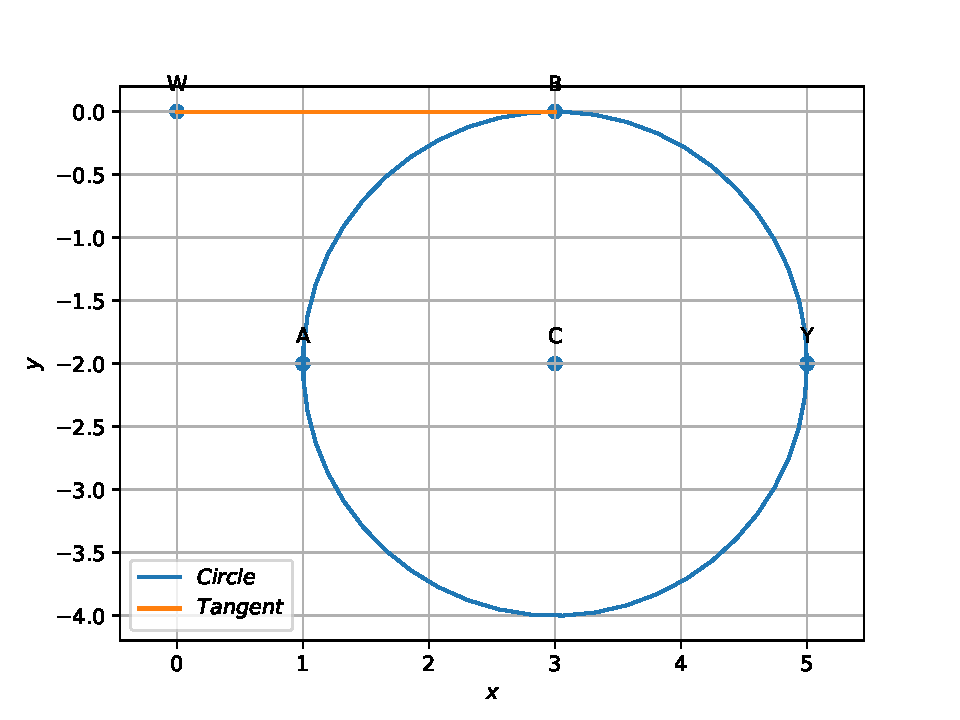
\includegraphics[scale=0.5]{cir.pdf}


\section{Problem}
The circle passing through $\myvec{1\\-2}$and touching the axis of x at $\myvec{3\\0}$ also passes through the point

A : $\myvec{-5\\2}$\\
B : $\myvec{2\\-5}$\\
C : $\myvec{5\\-2}$\\
D : $\myvec{-2\\5}$\\

\section{Solution}
\textbf{To find the center and Radius}
The equation of the circle is 
\begin{equation}
	x^T\vec{V}x + 2\vec{u}^Tx + f = 0
\end{equation}
Circle passes through $\myvec{1\\-2}$ 
\begin{equation}
	\vec{A}\vec{A}^T + 2\vec{u}^T\vec{A} + f = 0
\end{equation}
\begin{equation}
	\norm{A}^2 + 2\vec{A}^T \vec{u} + f = 0
\end{equation}
\begin{equation}
	\myvec{2\vec{A}^T & 1}\myvec{\vec{u} \\ f} = -\norm{A}^2 
\end{equation}
\begin{equation}
	\vec{B}\vec{B}^T + 2\vec{u}^T\vec{B} + f = 0
\end{equation}
\begin{equation}
	\norm{B}^2 + 2\vec{u}^T\myvec{B} + f = 0
\end{equation}
\begin{equation}
	\myvec{2B^T & 1}\myvec{\vec{u} \\ f} = -\norm{B}^2
\end{equation}
The equation of the tangent is
\begin{equation}
	\vec{m}^T (\vec{V}q + \vec{u}) = 0
\end{equation}
\begin{equation}
	\vec{m}^T\vec{B} +\vec{m}^T\vec{u} = 0
\end{equation}

$\vec{C} = -\vec{u}$  
\begin{equation}
	\myvec{\vec{m}^T & 0 \\ 2\vec{A}^T & 1 \\ 2\vec{B}^T & 1}\myvec{\vec{u} \\ f} = \myvec{-\vec{m}^T\vec{B} \\ -\norm{\vec{A}}^2 \\ -\norm{\vec{B}}^2}
\end{equation}
\begin{center}
	$\myvec{1&0&0&-3 \\2 & -4 & 1 & -9 \\ 6 & 0 & 1 & -5 } \xrightarrow[]{R_2 \leftarrow -2R_1 + R_2 } 
	\myvec{1&0&0&-3 \\0 & -4 & 1 & 1 \\ 6 & 0 & 1 & -9 } \xrightarrow[]{R_3 \leftarrow-6R_1 + R_3 } 
	\myvec{1&0&0&-3 \\0 & -4 & 1 & 1 \\ 0 & 0 & 1 & 9 } \xrightarrow[]{R_2 \leftarrow  R_2/4 } 
	\myvec{1&0&0&-3 \\0 & 1 & \frac{-1}{4} & \frac{-1}{-4} \\ 0 & 0 & 1 & 9 } \xrightarrow[]{R_2 \leftarrow \frac{1}{4}R_3+ R_2 } 
	\myvec{1&0&0&-3 \\ 0&1&0&2 \\ 0&0&1&9}$
\end{center}
By solving the above equations

The center is $\vec{C} = \myvec{3 \\ -2}$
 and $f = 9$ \\
\textbf{Radius}\\

\begin{equation}
	\vec{m} = \myvec{1\\-2} - \myvec{3\\-2} = \myvec{2\\0}
\end{equation}

\begin{equation}                                                                                   \sqrt{\myvec{2 &0}\myvec{2\\0}} = 2                                              
\end{equation}

from the given points $\myvec{5\\-2}$ satisfies the above condition
\begin{equation}
\vec{m} = \myvec{5\\-2} - \myvec{3\\-2} = \myvec{2\\0}
\end{equation}
\begin{equation}
	\sqrt{\myvec{2 &0}\myvec{2\\0}} = 2
\end{equation}
$\therefore \myvec{5\\-2}$ lies on the circle 
\end{document}

